%%%%%%%%%%%%%%%%%%%%%%%%%%%%%%%%%%%%%%%%%%%%%%%%%%%%%%%%%%%%%%%%%%%%%
% LaTeX Template: Project Titlepage Modified (v 0.1) by rcx
%
% Original Source: http://www.howtotex.com
% Date: February 2014
% 
% This is a title page template which be used for articles & reports.
% 
% This is the modified version of the original Latex template from
% aforementioned website.
% 
%%%%%%%%%%%%%%%%%%%%%%%%%%%%%%%%%%%%%%%%%%%%%%%%%%%%%%%%%%%%%%%%%%%%%%

\documentclass[12pt]{article}
\usepackage[a4paper]{geometry}
\usepackage[myheadings]{fullpage}
\usepackage{fancyhdr}
\usepackage{lastpage}
\usepackage{graphicx, wrapfig, subcaption, setspace, booktabs}
\usepackage[T1]{fontenc}
\usepackage[font=small, labelfont=bf]{caption}
\usepackage{fourier}
\usepackage[protrusion=true, expansion=true]{microtype}
\usepackage[english]{babel}
\usepackage{sectsty}
\usepackage{url, lipsum}
\usepackage{indentfirst}
\usepackage{graphicx}
\usepackage{float}
\usepackage{caption}
\usepackage{multirow}
\usepackage{enumerate}


\newcommand{\HRule}[1]{\rule{\linewidth}{#1}}
\onehalfspacing
\setcounter{tocdepth}{5}
\setcounter{secnumdepth}{5}


%-------------------------------------------------------------------------------
% HEADER & FOOTER
%-------------------------------------------------------------------------------
\pagestyle{fancy}
\fancyhf{}
\setlength\headheight{15pt}
\fancyhead[L]{EEE101 C Programming and Software Engineering 1}
\fancyhead[R]{Assessment 2 Report}
\fancyfoot[R]{Page \thepage\ of \pageref{LastPage}}
%-------------------------------------------------------------------------------
% TITLE PAGE
%-------------------------------------------------------------------------------

\begin{document}
	
	\title{ \normalsize \textsc{}
		\\ [2.0cm]
		\HRule{0.5pt} \\
		\LARGE \textbf{EEE101 C Programming Report\\Assessment 2}
		\HRule{2pt} \\ [0.5cm]
		\normalsize Nov 4, 2018 \vspace*{5\baselineskip}}
	
	\date{}
	
	\author{
		Name: Ziqi Yang\\
		ID: 1718112\\
	}
	
	\maketitle
	\newpage
	\tableofcontents
	\newpage
	
	%-------------------------------------------------------------------------------
	% Section title formatting
	%\sectionfont{\scshape}
	%-------------------------------------------------------------------------------
	
	%-------------------------------------------------------------------------------
	% Introduction
	%-------------------------------------------------------------------------------
	\section{Problem Statement}
	
	\subsection{Introduction}
	Provide an interface through which user can play a user determined number of games of rock, scissors, paper against the computer. The picture of characters user and computer select, current scores of user and computer will be display in each game. After chosen number of games have been played, the program will determine who is the final winner and output the result on screen, and ask user if to play again or exit the game. The limitations of the input data are as follows:
	
	\begin{enumerate}
	\item In welcome UI (to choose start or exit game), user can input "a" or "b".
	\item In information input UI, user can input name with any character but a full-space name, and game times number as a positive integer less than 50.
	\item In rounds UI, user can input "r"(rock), "s"(scissors) and "p"(paper) to represent the character they choose.
	\item In final UI, user can input "y" or "n" to decide whether to play again or not.
	\end{enumerate}

	\subsection{Inputs}
	If an illegal input is detected, the program will display the illegal input prompt for a few seconds, and then asks user to re-enter again. Being illegal input may be defined as follows:
	
	\begin{enumerate}
	\item In welcome UI: the input is not "a" or "b".
	\item In information input UI:
	
		\begin{enumerate}[1)]
		\item For the name input: the input is only consisting of space or nothing is input.
		\item For the game times input: the input is not a positive number less than 50.
		\end{enumerate}
	
	\item In rounds UI: the input is not "r", "s", or "p".
	\item In final UI: the input is not "y" or "n".
	\end{enumerate}

	\subsection{Outputs}
	The activities after each input are as follow:
	
	\begin{enumerate}
	\item If input is legal, go to the next step of the program.	
	\item If input is illegal, prompt user to re-enter.
	\end{enumerate}
	
	\subsection{Exit}
	After the game finished, ask user to choose play again or exit.

	%-------------------------------------------------------------------------------
	% Experimental Setup and Procedure
	%-------------------------------------------------------------------------------
	\section{Analysis}
	
	\subsection{On inputs}
	Firstly, a message needs to be printed on the screen to let the users know what data/action this program expects. Because the execution is not terminated immediately once an illegal input is detected, but need to ask user to input again. Therefore, the program should accept all kinds of data which user input, so that it can check the legality of all data.
	
	\subsection{On outputs}
	Because the data input by user cannot be predicted before they enter, the outputs are need to be discussed in two types of result, which are correct output with legal input and incorrect output with illegal input. The details of the two types of outputs will be shown as follows:
	
	\begin{enumerate}
		\item The inputs are legal and outputs are correct:
	
		\begin{enumerate}[1)]
			\item In welcome UI, it will display the program will start or exit depends on user choice.
			\item In information input UI, it will output nothing and go to next step.
			\item In rounds UI, it will output the score and picture of choice of computer and user.
			\item In final UI, it will output winner and display the program will start or exit depends on user choice.
		\end{enumerate}
		
		All of these outputs are needed to printed on the screen with clear text messages.
	
		\item The inputs are illegal and outputs are incorrect:
		
		Display the input is illegal and ask user to input again.
	\end{enumerate}

	\subsection{Data structure}
	
	\begin{enumerate}
		\item Enumerate:\\
		Four enumerate types are used to declare different types of constants and treat them as elements of different sets. The enumerate types defined in the program are as follows:
		
		\begin{enumerate}[$\bullet$]
			\item General$\_$Select: represent the character that computer or user choose.
			elements: rock, scissors, paper.
			\item Character$\_$Size: represent the size of character picture to print.
			elements: mini, normal.
			\item Game$\_$Player: represent the winner of current or final.
			elements: computer, user, none.
			\item General$\_$Result: represent the result of input legality check.
			elements: result$\_$OK(the input is legal), result$\_$Error(the input is illegal).
		\end{enumerate}
		
		\item Pointer:\\
		The definition pointer corresponds to the address of the variable (as a linear structure), and is passed as a parameter to the function to operate and process the value of the corresponding variable in the function, so that the value of the variable can be changed in the incoming function and read in a layer function.
		
		\item Array:\\
		Define array to organize and store several variables of the same type in an orderly fashion (as elements of sets). The array in the program is used to store user input and the coordinate of the points in character pictures.
		
		\item Some single data to save local variable data.
	\end{enumerate}

	\subsection{Algorithm}
	
	Rock, scissors and paper algorithm. These three characters are mutual restraint. The relationship among them is as Figure 1:
	
	\begin{figure}[H]
		\centering
		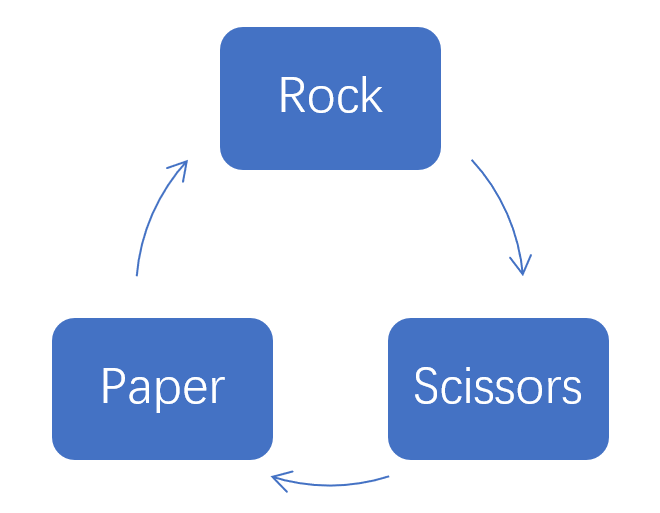
\includegraphics[width=2.5in]{Figure_1.png}
		\caption{Relationship among Rock, Scissors and Paper.}
	\end{figure}
	
	
	
	%-------------------------------------------------------------------------------
	% Results and Discussion
	%-------------------------------------------------------------------------------
	\section{Design}
	
	\subsection{Declare enumerate types}
		
		\begin{enumerate}
			\item General$\_$Select
			\item Character$\_$Size
			\item Game$\_$Player
			\item General$\_$Result
		\end{enumerate}
	
	\subsection{Go to welcome UI}
		
		\begin{enumerate}
			\item Display welcome messages to user.
			\item Ask user to choose start or exit.
		\end{enumerate}
		
	\subsection{Go to information input UI}
		
		\begin{enumerate}
			\item Ask user input name and do legality check.
			\item Ask user input game times and do legality check.
		\end{enumerate}
		
	\subsection{Go to rounds UI}
		
		\begin{enumerate}
			\item Display current score list and introduce to user that how to input.
			\item Ask user to input a character and do legality check.
			\item Generate a random number to generate what character the computer chooses.
			\item Display the picture of computer and user choose on screen.
			\item Compare the characters are chosen, give current winner and add the score.
			\item Display current winner this time.
			\item Ask user whether to continue game now.
			\item The remain game times minus 1.
			\item Repeat from step 1 to step 8 until all game times are consumed.
		\end{enumerate}
		
	\subsection{Go to final UI}
		
		\begin{enumerate}
			\item Compare scores of computer and user and judge the final winner.
			\item Display if the user winner.
			\item Ask user whether to play again.
		\end{enumerate}
		
	\subsection{Play again (repeat from 3.3 to 3.5) or exit.}
	
	%-------------------------------------------------------------------------------
	% Conclusion
	%-------------------------------------------------------------------------------
	\section{Implementation}
	See the C code "1718112$\_$2.c" with comments.
	
	%-------------------------------------------------------------------------------
	% Figures of Experiment Data Record
	%-------------------------------------------------------------------------------
	\section{Testing}
	
	\subsection{In welcome UI}
		
		\begin{enumerate}[$\bullet$]
			\item Input: a\\
			Return: text: The game will start!
			\item Input: b\\
			Return: text: The game will exit...
			\item Input: sdfgh (any character not "a" or "b")\\
			Return: text: Your input is illegal, please try again!
		\end{enumerate}
	
	\subsection{In information input UI}
		
		\begin{enumerate}[$\bullet$]
			\item Input: Ziqi Yang (any character but full-space)\\
			Return: (go to game times input).
			\item Input: (space of nothing)\\
			Return: text: The name cannot be space, please try again!
			\item Input: Ziqi Yang; 12(a positive integer less than 50)\\
			Return: (go to rounds UI).
			\item Input: Ziqi Yang; 0(a number not less than 50, a space, letters)\\
			Return: text: The times you input is illegal, please try again!
		\end{enumerate}
	
	\subsection{In rounds UI}

		\begin{enumerate}[$\bullet$]
			\item Input: r, s, p\\
			Return:
			\begin{enumerate}[1)]
				\item the character picture of computer and user chosen with character name below each picture
				\item text: Computer/User/Nobody win(s) this time!
				\item text: Press "Enter" to continue game...
			\end{enumerate}
		
			\item Input: sdf (anything is not r, s, p)\\
			Return: text: Your input is illegal, please try again!
		\end{enumerate}

	\subsection{In final UI}

		\begin{enumerate}[$\bullet$]
			\item Input: y\\
			Return: The game will start!
			\item Input: n\\
			Return: The game will exit...
			\item Input: asdf (anything is not y, n)\\
			Return: Your input is illegal, please try again!
		\end{enumerate}
	
\end{document}